\documentclass{article}
\usepackage{tikz}
\usetikzlibrary{shapes.geometric}

\begin{document}

\begin{figure}[h]
    \centering
    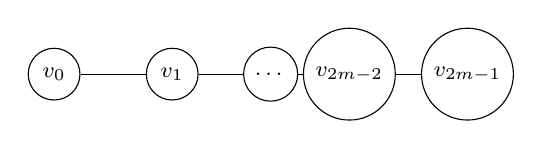
\begin{tikzpicture}[every node/.style={circle, draw}, font=\footnotesize]
        \node (v0) at (0, 0) {$v_0$};
        \node (v1) at (1.5, 0) {$v_1$};
        \node (vm2) at (3.75, 0) {$v_{2m-2}$};
        \node (vm1) at (5.25, 0) {$v_{2m-1}$};
        \node (vmid) at (2.75, 0) {\dots};

        \draw (v0) -- (v1);
        \draw (v1) -- (vmid);
        \draw (vmid) -- (vm2);
        \draw (vm2) -- (vm1);
    \end{tikzpicture}
    \caption{$P_{2m}$. The vertices $v_1$ through $v_{2m-2}$ each have two neighbors, while $v_{0}$ and $v_{2m-1}$ have one neighbor each. Thus, the vertices $v_1$ through $v_{2m-2}$ have maximal degree for this graph.}
    \label{fig:path}
\end{figure}

\end{document}